\documentclass[11pt,a4paper]{article}
% rozmery stranky
\usepackage[left=1.5cm,text={18cm, 25cm},top=2.5cm]{geometry}
% cestina a fonty
\usepackage[czech]{babel}
\usepackage[utf8]{inputenc}
\usepackage[T1]{fontenc}
% dalsi balicky
\usepackage{graphicx}
\usepackage{enumitem}
\usepackage{url}
\usepackage[bookmarksopen,colorlinks,plainpages=false,urlcolor=blue,
unicode,linkcolor=black]{hyperref}


\begin{document}

  \begin{titlepage}
    \begin{center}
      \Huge
      \textsc{Fakulta informačních technologií \\ Vysoké učení technické v~Brně}
      \vspace{100px}
      \begin{figure}[!h]
        \centering
        
\includegraphics[height=5cm]{logo}
      \end{figure}
      \\[50mm]
      \LARGE{Tvorba uživatelských rozhraní \,--\, projekt č. 93 \\
             Správa hostingu}
      \vfill
    \end{center}
    \Large{Roman Blanco (xblanc01) - kapitán týmu \hfill 24.10.2014 \\
           Adam Jež (xjezad00)}

  \end{titlepage}

  \section{Abstrakt}

    Cílem zadaného projektu je navrhnout a vytvořit uživatelské rozhraní,
    umožňující uživateli konfigurovat a spravovat své hostingové služby.
    Námi navržené rozhraní by mělo umožňovat správu FTP účtů, DNS
    záznamů, e-mailů a MySQL databází. Ovládání rozhraní navrhujeme tak, aby
    bylo přizpůsobeno jak uživatelům stolních počítačů, tak i uživatelům
    mobilních zařízení, které dokáží zobrazit internetový obsah. Protože naší
    snahou je maximální komfort zákazníků, nejčastěji užívané úkony by měly
    být lehce a rychle proveditelné.

  \section{Úvod}

    V~současnosti již existuje mnoho řešení uživatelských rozhraní pro správu
    hostingu.

    Při vyhledávání inspiračního materiálu jsme se zaměřili na vlastní práci s
    rozhraním - přehledost obsahu, způsob práce s daty a jejich řazení.
    Při návrhu vlastního rozhraní jsme se snažili vyvarovat případných chyb,
    které jsme nalézali v existujících řešeních. Z tohoto hlediska nám
    materiál poskytl jak pozitivní, tak i negativní inspiraci.  Jako studijní
    materiál nám sloužilo především rozhraní webhostingů roští.cz a wedos.cz \\
    \begin{figure}[ht]
      \begin{center}
        \includegraphics[width=12cm]{rosti}
        \caption{Uživatelské rozhraní webhostingu roští.cz}
      \end{center}
    \end{figure}
    \begin{figure}[ht]
      \begin{center}
        \includegraphics[width=12cm]{wedos}
        \caption{Uživatelské rozhraní webhostingu wedos.cz}
      \end{center}
    \end{figure}

  \section{Studium}

    Pro projekt plánujeme použít tyto technologie:
    \begin{description}
      \item[bower] technologie umožňující správu javascriptových knihoven
      \item[less] preprocesor pro CSS
      \item[charts.js] knihovna umožňující jednoduché vytváření grafů
      \item[MySQL] dotazovací jazyk pro získání informací spojené s~uživatelem
      \item[PHP] skriptovací jazyk běžně používaný pro programování
                   dynamických webových stránek
      \item[XML] značkovací jazyk pro popis dokumentu
      \item[XSL] jazyk pro vyjádření stylu
    \end{description}

  %\section{Návrh aplikace}

  \section{Návrh uživatelského rozhraní}

    Našim uživatelským rozhraním bychom chtěli zaujmout také amatérské
    klienty či zákazníky z~menších firem. Oslovit se je budeme snažit
    hlavně jednoduchým a uživatelsky příjemným prostředím se základními funkcemi.
    Naše uživatelské rozhraní by mělo být natolik přívětivé, aby
    jej dokázali ovládat a spravovat i méně zkušení klienti či přímo laici.
    Předpokládáme, že naše cílová skupina nebude zkušena natolik, aby si
    vytvořila vlastní analyzační nástroje, a proto chceme dát možnost použít, mimo jiné,
    užitečné statistiky související s~navštěvováním a používáním hostovaných
    webových stránek.

  \section{Realizace}

    Dosavadní práci na projektu jsme si rozdělili následujícím způsobem:
    \begin{description}
      \item[Roman Blanco] \hfill
        \begin{itemize}
          \item návrh vzhledu rozhraní
          \item zvážení technologií pro použití
          \item vyhledání a nastudování inspiračního materiálu
        \end{itemize}
      \item[Adam Jež:] \hfill
        \begin{itemize}
          \item návrh jednotlivých částí rozhraní
          \item návrh a vytvoření ERD podle návrhu rozhraní
          \item implementace logiky aplikace
        \end{itemize}
    \end{description}

    Klíčovou vlastností administrace webhostingu by měla být přehlednost. Snažili jsme se
    vytvořit prostředí tak, aby obsahovalo pouze potřebné prvky a neodvádělo
    pozornost uživatele k částem, se kterými v daném úkonu není třeba pracovat.

    K vytvoření přehledného prostředí jsme využili možnosti CSS/JS knihovny
    Twitter Bootstrap na všech vytvořených stránkách.
    Pro lepší znázornění dat jsme také, na stránce obsahující statistiky, použili
    JavaScriptovou knihovnu charts.js, která vytváří pohledné interaktivní grafy.

    Námi vytvořená administrace webhosingu obsahuje 4 hlavní části pro řízení
    webhostingu -- sekce pro správu FTP účtů, emailových schránek, MySQL databází
    a DNS záznamů. Další části jsou již zmíněné statistiky, s informacemi o
    uživatelích navštěvující hostovaný web. Vlastníkovi hostingu tyto informace
    mohou posloužit například k optimalizaci svého obsahu pro získání vyšší návštěvnosti.

    Poslední částí administrace webhostingu je sekce s nastavením, kde lze měnit přihlašovací
    údaje a notifikace systému, ale také zakoupit či prodloužit služby hostingu
    nebo získat podrobnější informace o již zakoupených službách.

    \subsection{Dosavadní implementace}

    Kostra webových stránek je připravena. Jednotlivé sekce, včetně stránky s přihlašováním jsou
    obsahově a funkčně hotové. Předpokládáme, že tyto části čekají už jen mírné kosmetické
    úpravy. Je potřeba se rozhodnout, co v zadání znamená pokyn vytvořit přepínání mezi více hostovanými doménami. 
    Musíme si ujasnit, jakým způsobem implementovat tuto funkci.

    V projektu aktuálně využíváme následující technologie:
    \begin{description}
      \item[charts.js] knihovna umožňující jednoduché vytváření grafů
      \item[AngularJS] knihovna umožňující vytváření interaktivnějších stránek
      \item[Twitter Bootstrap] JS/CSS framework pro urychlení a usnadnění vytváření vzhledu
      \item[BootstrapValidator] knihovna pro vytvareni interaktivnich formularu
      \item[MySQL] dotazovací jazyk pro získání informací spojené s~uživatelem
      \item[PHP] skriptovací jazyk běžně používaný pro programování
                   dynamických webových stránek
      \item[HTML] značkovací jazyk pro popis webovych stranek
      \item[CSS] jazyk definujici vzhled HTML elementu
      \item[XML] značkovací jazyk pro popis dokumentu
      \item[XSL] jazyk pro vyjádření stylu
    \end{description}

  \section{Testování}
  Dosavadní testování bylo prováděno pouze v rámci týmu. Následující závěrečné
  testování rozdělíme do dvou částí. 

  První část se skládá z vytvoření dotazníku, 
  který bude obsahovat taktéž úkoly pro dotazované. Dotazník pošleme širší skupině
  převážně studentů (jelikož jsme se na ně při vývoji zaměřili). Dotazník bude obsahovat otázky:
  
  \begin{itemize}
    \item Kolik je vám let?
    \item Jste studentem?
    \item Využíváte nějakých hostingových služeb, připadně jakých? Co vas zaujalo na první pohled?
  \end{itemize}

  Následuje řada úkonů

  \begin{itemize}
    \item Jaký máte z webhostingu pocit?
    \item Cítil jste se v nějakou chvíli ztracený?
    \item Měl jste s něčím v nějakou chvíli problém?
    \item Ohodnoťte, prosím, jak jste spokojený s webhostingem
    \item Ohodnoťte, prosím vzhled webhostingu.
    \item Dokázal byste takovýto system používat?
    \item Napadá vás, co by se dalo zlepšit?
  \end{itemize}

  Druha cast se sklada z osobniho pristupu k dotazovanym. Hlavnim prinosem tohoto pristupu 
  schledavame v podrobnejsim vystupu takovych to testu. Budou probihat podobne jak prvni, 
  s rozdilem, ze zadavatel testu bude merit trvani jednotlivych ukon a sledovat, kde uzivatel
  upira svuj pohled. Zda-li neprehlizi dulezite casti navigace, nebo zda-li se nedostal 
  do bodu, kde by se ztratil.

  Očekáváme, že výsledky testů nám potvrdí úspěch našich počátečních cílů. Zaměřili jsme se
  na jednoduchost, rychlost a přehlednost. Rádi bychom tedy, kdyby byl uživatel se 
  systémem spokojený, na pohled se mu líbil a práce s ním byla dostatečně efektivní a rychlá.
  Jelikož jsme použili minimum prvků, očekáváme také, že si uživatel rychle na systém
  zvykne a navigace v něm mu nebude dělat problém.

  %\section{Závěr}

  \section{Reference}

    \begin{enumerate}[label={[\arabic*]}]
      \item repoziář administrace serveru \href{https://github.com/creckx/pcp}{roští.cz}
      \item administrace serveru \href{https://wedos.cz}{wedos.cz}
    \end{enumerate}

  \appendix
  \newpage

  \section{Přílohy}

    \subsection{ERD}

    \begin{figure}[ht]
      \begin{center}
        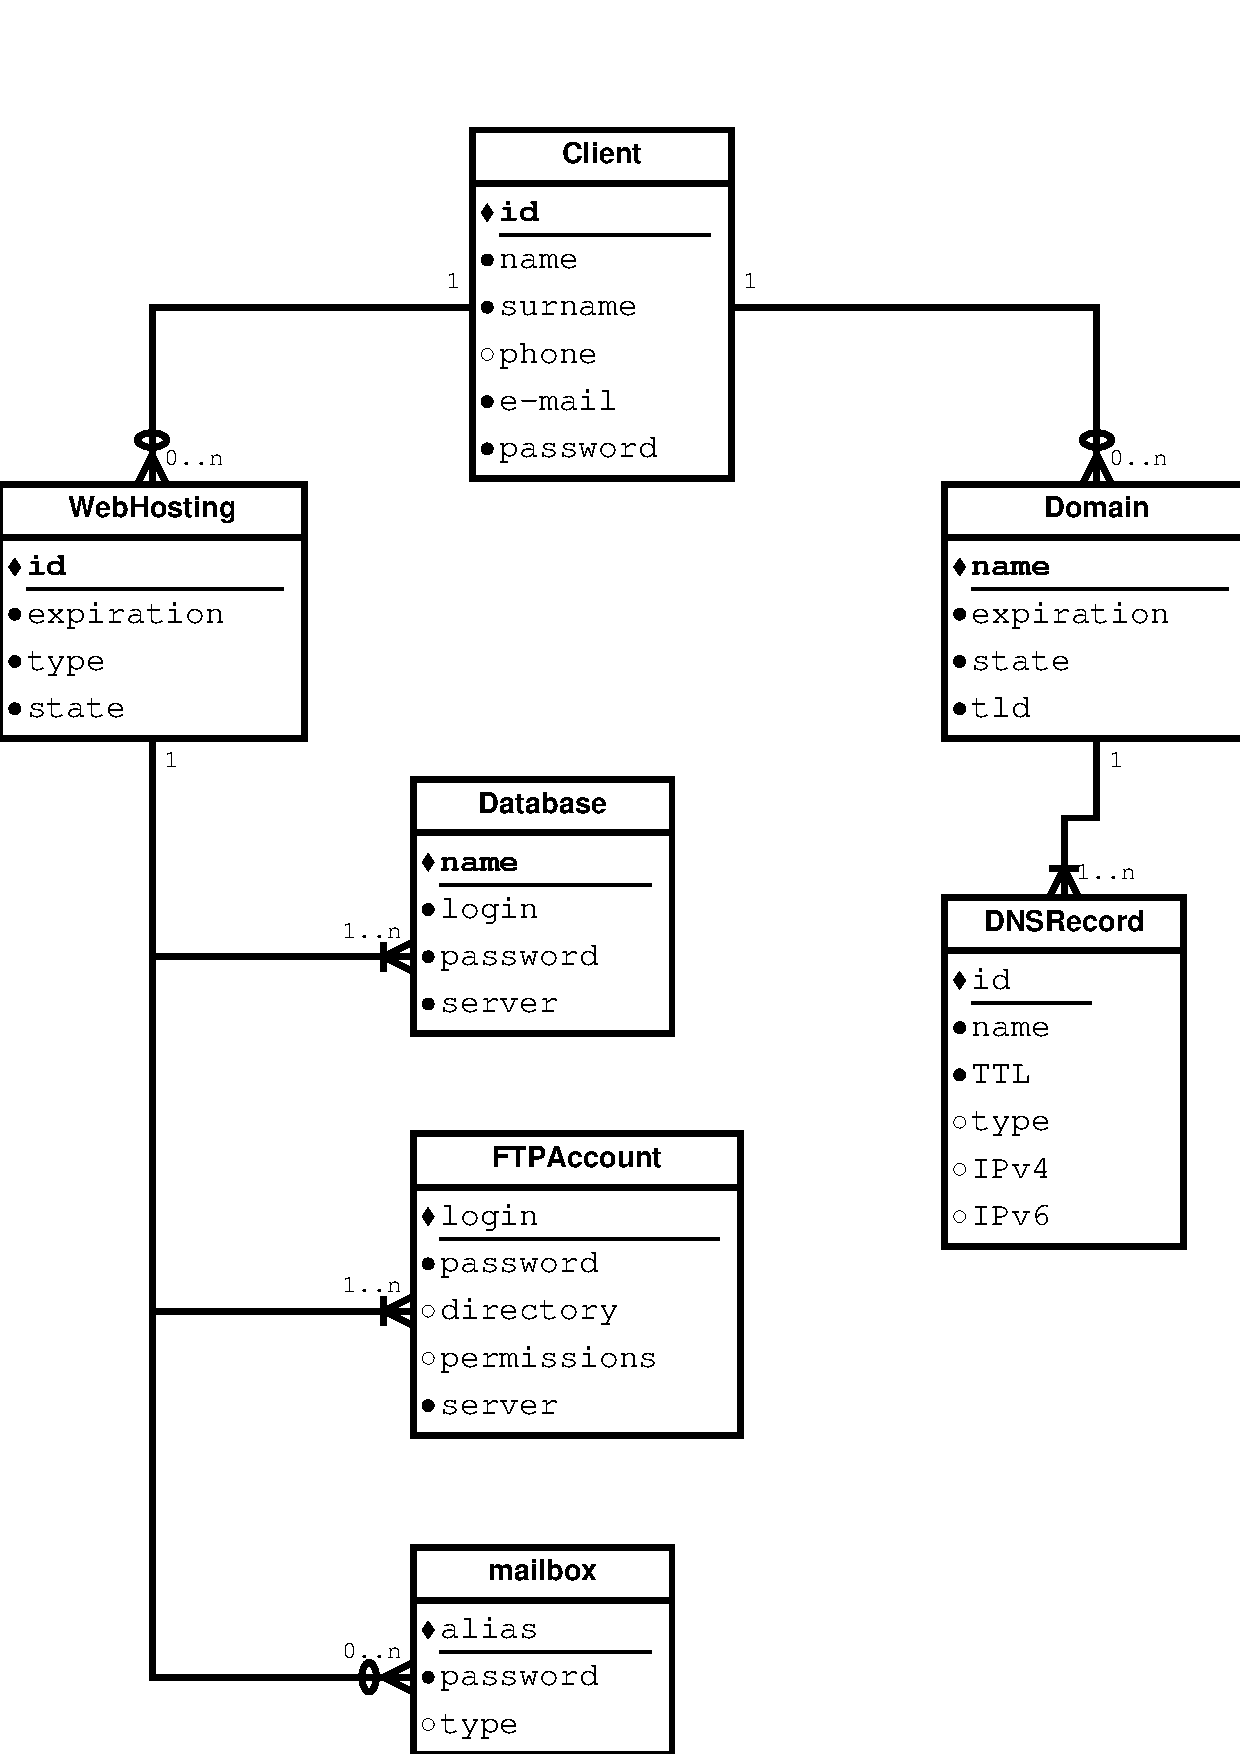
\includegraphics[width=10cm]{erd}
        \caption{ERD}
      \end{center}
    \end{figure}

\end{document}

